\newpage
\subsection{Declaring classes and attributes}
\texHeader
\hypertarget{static:classes tex}{}

% Discuss syntax in this section! (We removed it from Part I)
\begin{itemize}

\item[$\blacktriangleright$] Right click \texttt{LearningBoxLanguage}, and create your first EClass model by going to ``New/EClass.'' Name it `Box'.

\item[$\blacktriangleright$] The class editor should automatically open. Let's add the first two EAttributes of our program, \texttt{name} and
\texttt{stringRep}. In the MOSL syntax, attributes are declared by separating their name from their type. In this case, both are \texttt{EString} types
(Fig.~\ref{fig:boxDeclaration}).

\vspace{0.5cm}

\begin{figure}[htbp]
	\centering
  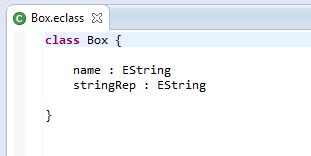
\includegraphics[width=0.5\textwidth]{eclipse_classBoxDeclaration}
	\caption{Newly created box class}
	\label{fig:boxDeclaration}
\end{figure} 

\vspace{0.5cm}

\item[$\blacktriangleright$] Create two more empty classes in your model, \texttt{Partition} and \texttt{Card}.

\item[$\blacktriangleright$] In \texttt{Partition}, add two \texttt{EInt} datatypes, \texttt{index} and \texttt{partitionSize}.

\item[$\blacktriangleright$] In \texttt{Card}, create three \texttt{EString}s, \texttt{back}, \texttt{face} , and \texttt{partitionHistory}.

\item[$\blacktriangleright$] If you've done everything correctly, the key areas in your workspace should now resemble Fig.~\ref{fig:workspaceClassAttributes}.

\item[$\blacktriangleright$] That's it for declaring class attributes! Feel free to build your project again and view the changes in the \texttt{.ecore}
mode, and the generated files in ``gen" and ``src." On a final note, while some languages (such as Java) allow the declaration of several small classes (such as
these three) in the same file, when tooling with eMolfon, it's best to have them separated. The MOSL builder will not give you an error if you implement them this way, but none of your program's dynamic actions will work. Don't worry - we'll explain this later in the handbook. As for now, continue to the next section to start creating references between these classes.

\newpage

\vspace*{3cm}

\begin{figure}[htbp]
	\centering
  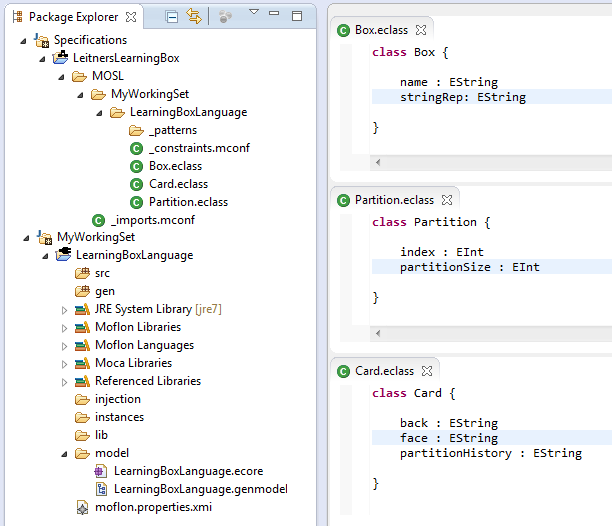
\includegraphics[width=1.0\textwidth]{eclipse_workspaceTexClassAttributes}
	\caption{Declaration of classes and attributes}
	\label{fig:workspaceClassAttributes}
\end{figure} 

% \fancyfoot[R]{$\triangleright$ \hyperlink{static:references splash}{Next}}

\end{itemize}
